%%%%%%%%%%%%%%%%%%%%%%%%%%%%%%%%%%%%%%%%%%%%%%%%%%%%%%%%%%%%%%%%%%%%%%%
%
%  A small sample UNSW Honours Thesis file.
%  Any questions to Ian Doust i.doust@unsw.edu.au
%
% Edited CSG 11.9.2015, use some of Gery's ideas for front matter; add a conclusion chapter.
%%%%%%%%%%%%%%%%%%%%%%%%%%%%%%%%%%%%%%%%%%%%%%%%%%%%%%%%%%%%%%%%%%%%%%%
%
%  The first part pulls in a UNSW Thesis class file.  This one is
%  slightly nonstandard and has been set up to do a couple of
%  things automatically
%
 
\documentclass[honours,12pt]{unswthesis}
\linespread{1}
\usepackage{cite}
\usepackage{amsfonts}
\usepackage{amssymb}
\usepackage{amsthm}
\usepackage{amsmath}
\usepackage{latexsym,amsmath}
\usepackage{graphicx}
\usepackage{afterpage}
\usepackage{tabularx}
\usepackage{hyperref}
\usepackage{algorithm}
\usepackage{algpseudocode}
\usepackage{float}
\usepackage{caption}
\usepackage{subcaption}
\usepackage{tikz}
\usetikzlibrary{arrows,matrix,positioning}

%%%%%%%%%%%%%%%%%%%%%%%%%%%%%%%%%%%%%%%%%%%%%%%%%%%%%%%%%%%%%%%%%
%
%  The following are some simple LaTeX macros to give some
%  commonly used letters in funny fonts. You may need more or less of
%  these
%
\newcommand{\R}{\mathbb{R}}
\newcommand{\Q}{\mathbb{Q}}
\newcommand{\C}{\mathbb{C}}
\newcommand{\N}{\mathbb{N}}
\newcommand{\F}{\mathbb{F}}
\newcommand{\PP}{\mathbb{P}}
\newcommand{\T}{\mathbb{T}}
\newcommand{\Z}{\mathbb{Z}}
\newcommand{\B}{\mathfrak{B}}
\newcommand{\BB}{\mathcal{B}}
\newcommand{\M}{\mathfrak{M}}
\newcommand{\X}{\mathfrak{X}}
\newcommand{\Y}{\mathfrak{Y}}
\newcommand{\CC}{\mathcal{C}}
\newcommand{\E}{\mathbb{E}}
\newcommand{\cP}{\mathcal{P}}
\newcommand{\cS}{\mathcal{S}}
\newcommand{\A}{\mathcal{A}}
\newcommand{\ZZ}{\mathcal{Z}}
%%%%%%%%%%%%%%%%%%%%%%%%%%%%%%%%%%%%%%%%%%%%%%%%%%%%%%%%%%%%%%%%%%%%%
%
% The following are much more esoteric commands that I have left in
% so that this file still processes. Use or delete as you see fit
%
\newcommand{\bv}[1]{\mbox{BV($#1$)}}
\newcommand{\comb}[2]{\left(\!\!\!\begin{array}{c}#1\\#2\end{array}\!\!\!\right)
}
\newcommand{\Lat}{{\rm Lat}}
\newcommand{\var}{\mathop{\rm var}}
\newcommand{\Pt}{{\mathcal P}}
\def\tr(#1){{\rm trace}(#1)}
\def\Exp(#1){{\mathbb E}(#1)}
\def\Exps(#1){{\mathbb E}\sparen(#1)}
\newcommand{\floor}[1]{\left\lfloor #1 \right\rfloor}
\newcommand{\ceil}[1]{\left\lceil #1 \right\rceil}
\newcommand{\hatt}[1]{\widehat #1}
\newcommand{\modeq}[3]{#1 \equiv #2 \,(\text{mod}\, #3)}
\newcommand{\rmod}{\,\mathrm{mod}\,}
\newcommand{\p}{\hphantom{+}}
\newcommand{\vect}[1]{\mbox{\boldmath $ #1 $}}
\newcommand{\reff}[2]{\ref{#1}.\ref{#2}}
\newcommand{\psum}[2]{\sum_{#1}^{#2}\!\!\!'\,\,}
\newcommand{\bin}[2]{\left( \begin{array}{@{}c@{}}
				#1 \\ #2
			\end{array}\right)	}
%
%  Macros - some of these are in plain TeX (gasp!)
%
\newcommand{\be}{($\beta$)}
\newcommand{\eqp}{\mathrel{{=}_p}}
\newcommand{\ltp}{\mathrel{{\prec}_p}}
\newcommand{\lep}{\mathrel{{\preceq}_p}}
\def\brack#1{\left \{ #1 \right \}}
\def\bul{$\bullet$\ }
\def\cl{{\rm cl}}
\let\del=\partial
\def\enditem{\par\smallskip\noindent}
\def\implies{\Rightarrow}
\def\inpr#1,#2{\t \hbox{\langle #1 , #2 \rangle} \t}
\def\ip<#1,#2>{\langle #1,#2 \rangle}
\def\lp{\ell^p}
\def\maxb#1{\max \brack{#1}}
\def\minb#1{\min \brack{#1}}
\def\mod#1{\left \vert #1 \right \vert}
\def\norm#1{\left \Vert #1 \right \Vert}
\def\paren(#1){\left( #1 \right)}
\def\qed{\hfill \hbox{$\Box$} \smallskip}
\def\sbrack#1{\Bigl \{ #1 \Bigr \} }
\def\ssbrack#1{ \{ #1 \} }
\def\smod#1{\Bigl \vert #1 \Bigr \vert}
\def\smmod#1{\bigl \vert #1 \bigr \vert}
\def\ssmod#1{\vert #1 \vert}
\def\sspmod#1{\vert\, #1 \, \vert}
\def\snorm#1{\Bigl \Vert #1 \Bigr \Vert}
\def\ssnorm#1{\Vert #1 \Vert}
\def\sparen(#1){\Bigl ( #1 \Bigr )}

\newcommand\blankpage{%
    \null
    \thispagestyle{empty}%
    \addtocounter{page}{-1}%
    \newpage}

%%%%%%%%%%%%%%%%%%%%%%%%%%%%%%%%%%%%%%%%%%%%%%%%%%%%%%%%%%%%%%
%
% These environments allow you to get nice numbered headings
%  for your Theorems, Definitions etc.  
%
%  Environments
%
%%%%%%%%%%%%%%%%%%%%%%%%%%%%%%%

\newtheorem{theorem}{Theorem}[section]
\newtheorem{lemma}[theorem]{Lemma}
\newtheorem{proposition}[theorem]{Proposition}
\newtheorem{corollary}[theorem]{Corollary}
\newtheorem{conjecture}[theorem]{Conjecture}
\newtheorem{definition}[theorem]{Definition}
\newtheorem{example}[theorem]{Example}
\newtheorem{remark}[theorem]{Remark}
\newtheorem{question}[theorem]{Question}
\newtheorem{notation}[theorem]{Notation}
\numberwithin{equation}{section}

%%%%%%%%%%%%%%%%%%%%%%%%%%%%%%%%%%%%%%%%%%%%%%%%%%%%%%%%%%%%%%%%%%
%
%  If you've got some funny special words that LaTeX might not
% hyphenate properly, you can give it a helping hand:
%
\hyphenation{Mar-cin-kie-wicz Rade-macher}

%%%%%%%%%%%%%%%%%%%%%%%%%%%%%%%%%%%%%%%%%%%%%%%%%%%%%%%%%%%%%%%%%%
% 
% OK...Now we get to some actual input.  The first part sets up
% the title etc that will appear on the front page
%
%%%%%%%%%%%%%%%%%%%%%%%%%%%%%%%%%%%%%%%%%%%%%%%%%%%%%%%%%%%%%%%%%

\title{Graph Learning Methods for Climate Models with Graph Sparsification}

\authornameonly{Justin Clarke}

\author{\Authornameonly\\{\bigskip}Supervisor: Associate Professor Yanan Fan}

\copyrightfalse
\figurespagefalse
\tablespagefalse

%%%%%%%%%%%%%%%%%%%%%%%%%%%%%%%%%%%%%%%%%%%%%%%%%%%%%%%%%%%%%%%%%
%
%  And now the document begins
%  The \beforepreface and \afterpreface commands puts the
%  contents page etc in
%
%%%%%%%%%%%%%%%%%%%%%%%%%%%%%%%%%%%%%%%%%%%%%%%%%%%%%%%%%%%%%%%%%%

\begin{document}

\graphicspath{ {C:/Users/jqcla/Documents/GitHub/Honours-Thesis/figures/} }

\beforepreface

\afterpage{\blankpage}

% plagiarism

\prefacesection{Plagiarism statement}

\vskip 10pc \noindent I declare that this thesis is my
own work, except where acknowledged, and has not been submitted for
academic credit elsewhere. 

\vskip 2pc  \noindent I acknowledge that the assessor of this
thesis may, for the purpose of assessing it:
\begin{itemize}
\item Reproduce it and provide a copy to another member of the University; and/or,
\item Communicate a copy of it to a plagiarism checking service (which may then retain a copy of it on its database for the purpose of future plagiarism checking).
\end{itemize}

\vskip 2pc \noindent I certify that I have read and understood the University Rules in
respect of Student Academic Misconduct, and am aware of any potential plagiarism penalties which may 
apply.\vspace{24pt}

\vskip 2pc \noindent By signing 
this declaration I am
agreeing to the statements and conditions above.
\vskip 2pc \noindent
Signed: Justin Clarke \hfill Date: 17/11/2023 \newline
\vskip 1pc

\afterpage{\blankpage}

% Acknowledgements are optional


\prefacesection{Acknowledgements}

% {\bigskip}By far the greatest thanks must go to my supervisor for
% the guidance, care and support they provided. 

% {\bigskip\noindent}Thanks 
% must also go to Emily, Michelle, John and Alex who helped by
% proof-reading the document in the final stages of preparation.

% {\bigskip\noindent}Although
% I have not lived with them for a number of years, my family also deserve
% many thanks for their encouragement.

% {\bigskip\noindent} Thanks go to Robert Taggart for allowing his thesis
% style to be shamelessly copied.

% {\bigskip\bigskip\bigskip\noindent} Fred Flintstone, 2 November 2015.

\afterpage{\blankpage}

% Abstract

\prefacesection{Abstract}

Graph sparification techniques for graph neural networks have traditionally been used to 
accelerate training and inference on real-world graphs which have billions of paramaters.
There are also many different climate models which use complex mathematical models to model 
the interactions between energy and matter over the world. Many of these models share 
components and the structure of these relationships is not easily found due to the complexity of
these climate models. The space of all possible graphs grows exponentially with the number 
of nodes and as such any correlation or causality is difficult to find. In this thesis, I attempt 
to quantify these relationships with graph sparsification techniques.
(Talk more about climate?)
\afterpage{\blankpage}


\afterpreface

%%%%%%%%%%%%%%%%%%%%%%%%%%%%%%%%%%%%%%%%%%%%%%%%%%%%%%%%%%%%%%%%%%
%
% Now we can start on the first chapter
% Within chapters we have sections, subsections and so forth
%
%%%%%%%%%%%%%%%%%%%%%%%%%%%%%%%%%%%%%%%%%%%%%%%%%%%%%%%%%%%%%%%%%%
\listoffigures
\listoftables

\afterpage{\blankpage}

\chapter{Introduction}\label{s-intro}

{\section{Climate Models}}\label{climate-introduction}

{\noindent}Climate models are based on well-known scientific processes and attempt to simulate the movement of fluids and energy throughout a system. 
The simplest of these have existed since the 1950's with the very first computers modelling simple variables on small two-dimensional climates\cite{edwards2011history}.
Modern Global Climate Models (GCMs) have been expanded to covering the globe in three dimensions. Most of these model the complex interactions between various physical, chemical, biological and geological processes. 
These models are constantly being updated with new data as many different groups and institutions implement higher spatial and temporal resolutions.
This has in part been driven by developments in computational techniques and the vast amount of data available worldwide to train these models.\cite{Overpeck2011}
A common approach to studying the complex system of Earth's climate has been through sophisticated mathematical modelling with a range of temporal and spatial data\cite{Kulinich_2022}
and at the centre of most of these approaches are the Navier-Stokes equations which are used describe the movements of liquids and gases in our oceans and atmosphere.\cite{Palmer2008} \\

{\noindent}The primary focus of these models has been forecasting time series data, as climate science aims to address a fundamental question: 
What impact have contemporary human greenhouse gas emissions had on the Earth and its future?
Understanding this is important as it can inform us on the potential harms to society and the environment and guide the population and policy makers who are implementing change.
The Coupled Model Intercomparison Project is a collaborative project between many meteoriological institutions that aims to improve our understanding of climate change.
The sixth iteration of these models or CMIP6 are the premier models for this task but while it was expected to contain around 100 models made by 49 separate groups, 
delays have caused only 40 have been published so far.
However, the results from these 40 models so far indicates a far greater sensitivity to increases in greenhouse gases when compared to the previous generation of CMIP5 models.\cite{Harrisson_2021}\\
% This suggests a far greater impact from the newer processes that were quantified in CMIP6. \\

{\noindent}The basis behind the Intergovernmental Panel on Climate Change and its 2021 IPCC sixth assessment from the Coupled Model Intercomparison Project (CMIP6) were the Shared Socioeconomic Pathways (SSP).\cite{lee2021future}
These SSP's represent a broad set of possible changes in population, economic and technological growth, and urbanisation that would influence future changes to the climte.\cite{RIAHI2017153}  
These are directly related to Representative Concentration Pathways (RCP) introduced by the previous CMIP5 which are categorisations based on the 
estimated future concentrations of greenhouse gases in the atmosphere.\cite{Harrisson_2021_SSP}.
Tables \ref{table:ssp} and \ref{table:rcp} detail the levels of these SSPs and RCPs.

\begin{table}[h]
    \centering
    \begin{tabularx}{\textwidth}{|c|X|}
        \hline
        \textbf{SSP} & \textbf{Description}                                                                                                                                                                                                                                                                      \\ \hline
        SSP1         & Sustainability: The world shifts gradually, but pervasively, toward a more sustainable path, emphasizing more inclusive development that respects perceived environmental boundaries.                                                                                                     \\ \hline
        SSP2         & Middle of the road: The world follows a path in which social, economic, and technological trends do not shift markedly from historical patterns.                                                                                                                                          \\ \hline
        SSP3         & Regional rivalry: A resurgent nationalism, concerns about competitiveness and security, and regional conflicts push countries to increasingly focus on domestic or, at most, regional issues.                                                                                             \\ \hline
        SSP4         & Inequality: Highly unequal investments in human capital, combined with increasing disparities in economic opportunity and political power, lead to increasing inequalities and stratification both across and within countries.                                                           \\ \hline
        SSP5         & Fossil-fueled development: This world places increasing faith in competitive markets, innovation and participatory societies to produce rapid technological progress and development of human capital as the path to sustainable development. Global markets are increasingly integrated. \\ \hline    
    \end{tabularx}
    \vspace{1pt}
    \caption{Shared Socioeconomic Pathways Descriptions}
    \label{table:ssp}
\end{table}

\begin{table}[ht]
    \centering
    \resizebox{\textwidth}{!}{\begin{tabular}{|c|c|c|}
        \hline
        \textbf{RCP} & \textbf{Temperature Increase (2081--2100)} & \textbf{Sea Level Rise (2081--2100)} \\ \hline
        2.6          & 1.0{\textdegree} C                                  & 0.4m                                   \\ \hline
        4.5          & 1.8{\textdegree} C                                  & 0.47m                                 \\ \hline
        6.0          & 2.2{\textdegree} C                                  & 0.48m                                  \\ \hline
        8.5          & 3.7{\textdegree} C                                  & 0.63m                                  \\ \hline
    \end{tabular}}
    \vspace{1pt}
    \caption{Representative Concentration Pathways}
    \label{table:rcp}
\end{table}

{\noindent}Scenarios are named based on the conjunction of their SSP level and RCP values. 
For example, on the lower end, SSP126 assumes an increasingly sustainable world where consumption is oriented towards 
minimising material resource and energy usage while SSP585 assumes a worst case scenario where fossil fuel usage and an energy-intensive lifestyle intensifies.
The main output of CMIP6 models are the ``scenario runs'' which predict various outcomes in temperature, precipitation, air pressure and solar radiation given a certain SSP over time from 1850--2100.

{\section{Ensemble Models}}\label{ensemble}

{\noindent}Ensemble modelling is a process where multiple models are used in combination for a task and are more performant when the base models are diverse and independent\cite{KOTU201919}.
Simple averages of multiple models are regularly shown to have better correlation with historical observations than any individual model alone.\cite{kharin2002climate}\cite{feng2011comparison}
CMIP6 is known as an `ensemble of opportunity'\cite{Knutti2010}, where the makeup the ensemble is determined by the ability of each base model to contribute.\cite{ClimateModelDependenceandtheEnsembleDependenceTransformationofCMIPProjections}
This is the main benefit of ensemble methods as models can be weighted based on how accurate they are certain predictions.
However, as research has become far more interconnected in the modern era, many aspects such as expertise, code and literature are often shared between groups. 
As such, many of the models that contribute to CMIP6 are highly likely to be dependent of each other.\cite{ClimateModelDependenceandtheEnsembleDependenceTransformationofCMIPProjections}. 
The degree of dependence between these models is difficult to ascertain as this would require a qualitative investigation into the personel, code and references between each component of CMIP6.
Various novel approaches such as stochastic Markov chains\cite{Kulinich_2022} have been used to provide a more optimal ensemble mean which may account for this dependence.
However, one would expect there to be some ground truth graph structure that links all models together through some dependence.

{\section{Machine Learning}}\label{ml}

{\noindent}The size of climate data has lead us to explore more scalable techniques to model this data.
There are many different kinds of machine learning but the advent of the deep learning paradigm in the past decade has become the gold-standard of machine learning\cite{alzubaidi2021review}.
This has led to countless advancements in many practical applications such as, audio processing\cite{adeel2020contextual}, visual data processing\cite{tian2020evolutionary} and natural language processing\cite{young2018recent} to name a few examples.
The name deep learning refers to the ability of deep learning models to extract high-level, abstract features from raw data by using many layers of simple, computer understandable representations.
Computers perform well on complex logical tasks such as arithmetic but often stuggle with more simplistic tasks that are harder to quantify such as visual recognition and language. 
The ability of deep learning models to quantify these simple tasks have allowed artifical intelligence to apporach near human level understanding.\cite{Goodfellow-et-al-2016} 
The first neural networks developed in the late 1950's sought to simulate how human brain learned and operated.\cite{Rosenblatt_1958}
The next development in neural networks also came from neuroscientific principles\cite{Hubel_Wiesel_1962} with Convolutional Neural Networks (CNN) which could train models to be equivariant to translations in data and process data with grid-like structure. 
In recent years, Graph Neural Networks (GNN) have become the premier method of processing data with non-cartesian structure as standard convolutions on a graph structure much harder to define.
The main feature of GNNs is the message passing framework, where information from features on each node is passed to neighbouring nodes then aggregated and embedded. 
This is then propagated through a neural network structure to perform a range of tasks on the entire graph, individual nodes or edges.
Much of this data exists in the world in applications such as chemical analysis\cite{xu2022chemistry}, social networks analysis\cite{rath2020detecting}, link prediction\cite{zhang2020revisiting} and unstructured data processing\cite{nouri2021improving}.

{\section{Sparsification of Deep Learning}}\label{sparsification}

An estimated 80 to 90 percent of the worlds' 79 zetabytes of data is unstructured and graphs make up a significant proportion of this data\cite{inmon2007tapping}.
Traditional neural networks are not able to extract meaninful insights from this unstructured data without significant cleaning.
The modern age has also produced many advancements in computing such as Massively Parallel Processing (MPP)\cite{nordstrom1992using} 
and big data which has led to an exponential growth in the size and complexity of these deep learning models.
The well-known Generative-Pretrained Transformer 3 (GPT-3) model by OpenAI commonly used for ChatGPT had variants with 175 billion parameters which required 800 gigabytes to store.\cite{radford2018improving}
Although Deep Neural Networks (DNN) tend to generalise well even when overparameterised\cite{Cao_Gu_2020}, this level of overparameterisation makes inference 
and prediction highly costly when the same performance could be achieved on a far more simple model. To address this, the concept of the
Lottery Ticket Hypothesis (LTH)\cite{frankle2020linear} was introduced which explored the possibility of simplifying redundant models by trainable sparse subnetworks whilst still training to full accuracy.
Chen et.al.\cite{chen2021unified} extended the LTH to Graph Neural Networks by co-optimising graph and neural networks weights and zeroing out edges with the lowest magnitude. 
This reduced computational costs by over 85\% depending on the size of the graph whilst maintaining a strong baseline accuracy.

{\section{Motivation}}\label{motivation}

The goal of this thesis is to investigate whether these graph sparisifcation techniques can be used to determine some dependence structure within a graph of models which
are all attempting to model the same scenario in the climate. Graph structure and dependence learning is already possible with unsupervised methods such as Variational Graph Autoencoders (VGAE)\cite{pmlr-v97-yu19a}
but to our best knowledge, graph sparsification has not been used before as a method for graph structure learning or infering dependence. Existing methods for determining multiple correlation such as 
partial correlation and multiple correlation coefficient $R^2$ are linear methods. Graph sparsification is primarily used for simplifying graphs which have been overparameterised and grown too large but 
by removing these edges, the edges that remain should theoretically hold some relation in dependence to the graph which is the motivation for this thesis.

{\section{Outline}}\label{outline}

{\noindent}The thesis is structured as follows. 
In Chapter 2, we will review the studies relating to neural networks, the extensions towards graph neural networks and the lottery ticket hypothesis (LTH).
Current methods along with the benefits and shortcomings will be discussed and the terminology and definitions for will also be outlined in this section. \\

{\noindent}In Chapter 3, we will perform an exploratory data analysis (EDA) and provide a high-level overview of the dataset. This will provide a more
in-depth understanding of the scenarios and CMIP6 models. There will also be a more comprehensive analysis of an individual climate modeL? (pick an example?)
the climate modelling process and ensemble weighting method? We then introduce our problem formulation with by formalising the regression problem we will be using
to perform the sparsification algorithm. \\

{\noindent}In Chapter 4, we visualise the results of the sparsification algorithm and we compare it to various correlation and partial correlation matrices. 
We may also look at Mutual Information Criterion (MIC) and compare with Variational Graph Autoencoder? \\

{\noindent}Finally in Chapter 5, we summarise our findings and present some directions for possible future research.


%%%%%%%%%%%%%%%%%%%%%%%%%%%%%%%%%%%%%

\chapter{Methods and Related Techniques}

%%%%%%%%%%%%%%%%%%%%%%%%%%%%%%%%%%%%%


% In this chapter we will give a brief overview on how the climate works and review 
% current standards in climate modelling along with the basics
% behind neural networks and the extensions towards graph neural networks.

% This will basically be the section on literature review. Current methods and techniques being
% used etc. A lot of summaries of the papers saved in the papers folder need to be done to 
% finish this section.


%%%%%%%%%%%%
\section{Deep Learning}\label{dl}
%%%%%%%%%%%%
The advent of deep learning provided algorithms that could automatically extract higher-level features from raw data.\cite{deng-deep-learning}
The multi-layer perceptron\cite{rumelhart1986learning} is formulated using linked layers of nodes which transforms a set of inputs into an output.
The single layer version of this model can be represented as

\begin{equation}
    f(x) = \sigma(\Theta^\top X)  \; \text{where}  \; \Theta= \begin{bmatrix} b \\ \theta_1 \\ \vdots \\ \theta_n \end{bmatrix} \text{and} \; X = \begin{bmatrix} 1 \\ x_1 \\ \vdots \\ x_n \end{bmatrix}
\end{equation}

\noindent Where $\sigma(.)$ is some activation function such as ReLu, hyperbolic tangent or logistic function, $X$ is the data, $\Theta$ is the learned parameters and $b$ represents a bias term.
These parameters are set to some initial values and are iteratively updated in a back-propagation training process,

\begin{equation}
    \theta^{t+1} = \theta^{t} - \eta\frac{\partial E(X, \theta^t)}{\partial\theta}
\end{equation}

\noindent Where $E(.)$ is some loss function and $\eta$ is the learning rate. \\

\noindent The next advancement in the deep learning space came with the Convolutional Neural Network (CNN) which was a regularised MLP that could
handle data with data with structure and multiple dimensions far better than the traditional MLP due to its use of weight sharing, 
sampling and local receptive fields.\cite{Goodfellow-et-al-2016}
Suppose we have an image or some other kind of data in two-dimensional matrix form. Let $\textbf{X} \in \mathbb{R}^{H\times W}$ be the input image and
$\textbf{W} \in \mathbb{R}^{h\times w}$ be the kernel or filter. By performing a convolution, we are effectively 'sliding' our weight matrix kernel
over our input and the resulting feature map $\textbf{Z} = \textbf{X} \ast \textbf{W}$,

\begin{equation}
    Z_{i, j} = \sum_{u=0}^{h-1}\sum_{v=0}^{w-1} x_{i+u, j+v} w_{u, v}
\end{equation}

\noindent The novelty of the convolutional layer compared to a linear layer is that the kernel is shared across all locations of the input and therefore
if a pattern in the input moves, the corresponding output will also follow this movement. This provides shift equivariance which is something that early MLP's
failed to achieve.\cite{pml1Book}

%%%%%%%%%%%%
\section{Graph Neural Networks}\label{gnn}
%%%%%%%%%%%%
When it comes to data in a graph-like structure, standard CNN's cannot be applied due to the non-euclidean nature of a graph.
In an image or a matrix, our kernel is generally a $n\times n$ matrix which can be applied to the entirety of the data. In graphs
this is not always possible due to the fact that any number of nodes can be connected by any number of edges.\cite{sanchez-lengeling2021a} \\

\begin{figure}[H]
    \centering
    \begin{subfigure}{\textwidth}
        \centering
        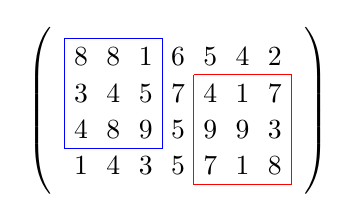
\begin{tikzpicture}
            \matrix [matrix of math nodes,left delimiter=(,right delimiter=)] (m)
            {
                8 &8 &1 &6 &5 &4 &2\\               
                3 &4 &5 &7 &4 &1 &7\\               
                4 &8 &9 &5 &9 &9 &3\\
                1 &4 &3 &5 &7 &1 &8\\
            };  
            \draw[color=blue] (m-1-1.north west) -- (m-1-3.north east) -- (m-3-3.south east) -- (m-3-1.south west) -- (m-1-1.north west);
            \draw[color=red] (m-2-5.north west) -- (m-2-7.north east) -- (m-4-7.south east) -- (m-4-5.south west) -- (m-2-5.north west);
        \end{tikzpicture}
        \caption{ }
        \label{fig:matrix_convolution}
    \end{subfigure}
    \hspace{3pt}
    \begin{subfigure}{.5\textwidth}
        \centering
        \includegraphics[width=\textwidth]{graph conv}
        \caption{ }
        \label{fig:graph_convolution}
    \end{subfigure}
    \caption{Examples of (a) matrix convolution with a $3\times 3$ kernel and (b) a graph where a convolution is much more difficult to define.}
    \label{fig:graph_conv_difficulty}
\end{figure}


{\noindent}The Graph Neural Network (GNN) was developed for this purpose and they can be broadly categorised into gating and attention based methods\cite{veličković2018graph} 
and spectral or spatial methods within Graph Convolutional Network (GCN) research.\cite{kipf2017semisupervised} \\

{\noindent}We define a graph as ${\mathcal{G}} = ({\mathcal{V}}, \textbf{A})$, where $\mathcal{V}$ represents a set of verticies which contains a list of nodes
$\{ v_1, \dots, v_n \}$ and $\textbf{A} \in \mathbb{R}^{n \times n}$ the adjacentcy matrix which contains information on the graph topology.
If an edge is also weighted from node $j$ to $i$, it is noted as $e_{ji}$.
If an edge exists between two node $v_i$ and $v_j$, then $\textbf{A}_{ij} = 1$ else, $\textbf{A}_{ij} = 0$. 
We also define the degree matrix as $\mathbf{D} = \sum_{j}A_{ij}$ where each entry on the diagonal is equal to the row sum of the adjacency matrix $\textbf{A}$.  
Each node has a {p}-dimensional feature vector ${x_i} \in \mathbb{R}^{p}$ which describes some information about the node in the graph. 
By combining all ${n}$ feature vectors from all nodes, we have a feature matrix $\textbf{X} \in \mathbb{R}^{n\times p}$. 
The graph also has a response ${Y} \in \mathbb{R}^p$ which is for a graph-level task but a node level task would simply have ${Y} \in \mathbb{R}^{n\times p}$.
The convolution operation from\cite{kipf2017semisupervised} can be expressed as

\begin{equation}
\mathbf{X'} = \tilde{D}^{-1/2} (A + I) \tilde{D}^{-1/2} \textbf{X} \Theta
% \sigma_2( \mathbf{ \hat{A} }_2 \sigma_1 (\mathbf{ \hat{A} }_1 \mathbf{X} \Theta^{(0)}) \Theta^{(1)})
\end{equation}

\noindent or on a nodel-level, the operation known as the message passing framework can be thought of as

\begin{equation}
    x'_i = \Theta^\top \sum_{j\in \mathcal{N}(i) \cup \{i\}} \frac{e_{ji}}{\sqrt{\hat{g}_j \hat{g}_i}} x_j.
\end{equation}

\noindent where $e_{ij}$ is the edge weight between nodes $i$ and $j$ and $\mathcal{N}(i)$ are the neighbouring nodes connected by an edge to node $i$. 
$\hat{g}_i = \sum_{j\in \mathcal{N}(i) \cup \{i\}} e_{ji}$ is the row sum of the the edge weights.
This effectively takes the node embeddings from each neighbouring node and aggregates it by a permutation invariant function such as the sum. 
Over many layers this passes the signal from all nodes around the graph to each other.\cite{sanchez-lengeling2021a}
The final learning function for a two layer network is then just

\begin{equation}
    f(\mathbf{A, X}) = \sigma_2( \mathbf{ \hat{A} }_2 \sigma_1 (\mathbf{ \hat{A} }_1 \mathbf{X} \Theta^{(0)}) \Theta^{(1)})
\end{equation}
where $\sigma_1(.)$ and $\sigma_2(.)$ are an activation function such as ReLU, and $\hat{A} = \tilde{D}^{-1/2} (A + I_N) \tilde{D}^{-1/2}$
is the symmetrically normalised adjacency matrix. The propagation rule is then as follows:

\begin{equation}
    H^{(l+1)} = \sigma(\tilde{D}^{-\frac{1}{2}} \tilde{A} \tilde{D}^{-\frac{1}{2}} H^{(l)} \Theta^{(l)})
\end{equation}

\noindent Here, $\tilde{A} = A + I_N$ is the adjacency matrix of the undirected graph $\mathcal{G}$ with self-connections from the identity matrix $I_N$.
$\tilde{D_{ii}} = \sum_{j} \tilde{A}_{ij} $ is the row sum of $\tilde{A}$ and $\Theta^{(l)}$ is a layer trainable weight matrix. 
$H^{(l)} \in \mathbb{R}^{N \times D}$ is the matrix of activations in the lth layer with $H^0 = \textbf{X}$ or the input. 


\section{Sparsification of Graph Neural Networks}\label{sparse-learning}

Hornik\cite{HORNIK1991251} showed that in a single layer MLP and provided enough hidden neuron units, 
the neural network could model any smooth truth function as for each added neuron, 
the decision space can be segmented to added linear regions to conform to any response. 
Many experiments have also found that deep networks with many layers perform better than shallow ones\cite{NIPS2014_109d2dd3}\cite{pmlr-v70-raghu17a}
as the usage of many layers allows deeper layers to leverage features produced by earlier layers.
The noveltly of neural networks is that they do not tend to be affected greatly by overparameterisation\cite{Cao_Gu_2020}, and as they generally improve with more neurons
and layers these models have grown exponentially in size with some models using billions of parameters and most of these models having more parameters than training observations
which has made both inference and prediction incredibly costly.  (Reference some math from the number of linear decision regions and some graphs?) \\

{\noindent}The most basic approach to inducing model sparsity is through an $l_1$ penalty also known as LASSO in the loss function.\cite{pml1Book}
Unlike the $l_2$ regularisation which penalises large magnitude weights, the $l_1$ regularisation minimises and zeros weights which encourages sparsity.
On a linear regression, this is done with a MAP estimation with a Laplace prior and is equivalent to optimising

\begin{equation}
    \mathcal{L}(\Theta) = \frac{1}{2}||\textbf{Y} - \textbf{X}\Theta||^2_2 + \lambda||\Theta||_1
\end{equation}

{\noindent}where $\lambda > 0$ is some tunable sparsity parameter.
This is a form of the bridge estimator\cite{frank1993statistical} where $\alpha = 1$ and $\Theta$ is a solution to the objective function

\begin{equation}
    \underset{\Theta}{\operatorname{argmax}} \frac{1}{2}||\textbf{Y} - \textbf{X}\Theta||^2_2 + \lambda \sum_{j=1}^{p} |\theta_j|^\alpha
\end{equation}

{\noindent}where $0 < \alpha < 1$. This bridge penalty induces the exponential power prior distribution on $\Theta$ in the form
\begin{equation}
    \pi(\Theta | \lambda, \alpha) = \propto \prod_{j=1}^{p} \frac{\lambda^{1/\alpha}}{2\Gamma(1 + 1/\alpha)} \exp(- \lambda |\theta_j|^\alpha)
\end{equation}

{\noindent}This is easily extended to neural networks by applying this penalty to the weights in the layers of the network.\cite{ma2019transformed}
Despite the this benefit, modern GPUs are optimised for dense matrix multiplication and as such there aren't many computational benefits from regularisation if certain weights across the network are zero.
Methods that encourage \textit{group} sparsity are able to prune whole nodes and layers out of our model result in \textit{block sparse} weight matricies which provide much more substanial computational savings.
\cite{scardapane2017group}\cite{wen2016learning}\cite{molchanov2017variational}\cite{louizos2017bayesian} \\

{\noindent}Dropout\cite{srivastava2014dropout} is another strategy traditionally used to prevent overfitting but has been formalised as structured shrinkage prior.\cite{nalisnick2019dropout}
At each training iteration, we turn off all outputs from each neuron with probability $p$. 
In this way, each neuron is trained to learn well individually even if some neurons are missing and prevents units from overfitting and depending on each other. 
We can view this as estimating a noise version of the weights\cite{pml1Book},

\begin{equation}
    \theta_{lji} = w_{lji}\epsilon_{li} \text{ where } \epsilon_{li} \sim Ber(1-p)
\end{equation}

{\noindent}When testing, this dropout is generally turned off but if used at test time, this becomes an ensemble of networks each with sparse graphs\cite{gal2016dropout}\cite{kendall2017uncertainties} 
and becomes Monte Carlo dropout. This can be expressed as

\begin{equation}
    p(\textbf{Y} | \textbf{X}, \mathcal{D}) \approxeq \frac{1}{N} \sum_{n=1}^{N}{p(\textbf{Y} | \textbf{X}, \hat{W}\epsilon^n+\hat{\textbf{b}})}
\end{equation}

{\noindent}The Lottery Ticket Hypothesis (LTH)\cite{frankle2020linear} explored the possibility of simplifying redundant models by trainable sparse subnetworks whilst
still training to full accuracy. Chen et. al.\cite{chen2021unified} extended the LTH to Graph Neural Networks by co-simplifying both the adjacentcy matrix of the graph and the weights in 
the network of the model. For a semi-supervised classification task, the objective function is:

\begin{equation}
    \mathcal{L}(\mathcal{G}, \Theta) = -\frac{1}{|\mathcal{V}_{\text{label}}|}\sum_{v_i \in \mathcal{V_{\text{label}}}} y_i \log{(z_i)},
\end{equation}
where $\mathcal{L}$ is the cross-entropy error of all samples and $y_i$ is the label vector of node $v_i$. The Unified GNN Sparsification (UGS)
framework then introduced two masks $m_g$ and $m_\theta$ with the same shape as the adjacency matrix $\textbf{A}$ and the weights matrix $\Theta$, which
gives the following objective function:

\begin{equation}\label{eqn:l_ugs}
    \mathcal{L}_{\text{UGS}} = \mathcal{L}(\{m_g \odot A, \textbf{X}\}, m_\theta \odot \Theta) + \gamma_1 ||m_g||_1 + \gamma_2 ||m_\theta||_1,
\end{equation}

\noindent where $\odot$ is the element-wise product, $\gamma_1$ and $\gamma_2$ are hyperparameters to control the shrinkage of $m_g$ and $m_\theta$.
After training, the lowest magnitude elements in $m_g$ and $m_\theta$ are set to zero with respect to some set values of $p_g$ and $p_\theta$.
These sparse masks are then applied which prune $\textbf{A}$ and $\Theta$. The algorithm is then as listed in Algorithm \ref{alg:ugs} and \ref{alg:iterative_ugs}

\begin{algorithm}
    \caption{Unifed GNN Sparsification\cite{chen2021unified}}\label{alg:ugs}
    \textbf{Input:} \text{Graph} $\mathcal{G} = \{A, \textbf{X}\}$, GNN $f(\mathcal{G}, \Theta_0)$, weight initialisation $\Theta_0$, masks $m^0_g = A$ and $m^0_\theta = 1 \in \R^{||\Theta_0||_0}$, step size $\eta, \lambda_g$ and $\lambda_\theta$,
    preset ratios $p_g$ and $p_\theta$\\
    \textbf{Output:} Sparse masks $m_g$ and $m_\theta$
    \begin{algorithmic}[1]
        \For{iteration $i = 0, 1, 2, \dots, N-1$}
            \State{Forward $f(\cdot, m^i_\theta \odot \Theta_i)$ with $\mathcal{G}=\{m_g^i\odot A, \textbf{X}\}$ \Comment{Computes \ref{eqn:l_ugs}}}
            \State{Backpropagate to update $\Theta_{i+1} \gets \Theta_i - \eta \nabla_{\Theta_i} \mathcal{L}_{UGS} $}
            \State{Update $m_g^{i+1} \gets m_g^i - \eta \nabla_{m_g^i} \mathcal{L}_{UGS}$}
            \State{Update $m_\theta^{i+1} \gets m_\theta^i - \eta \nabla_{m_\theta^i} \mathcal{L}_{UGS}$}
        \EndFor
        \State Set $p_g$ of the lowest magnitude values in $m_g^N$ to 0 and others to 1, then obtain $m_g$. \Comment{Set at $5\%$}
        \State Set $p_\theta$ of the lowest magnitude values in $m_\theta^N$ to 0 and others to 1, then obtain $m_\theta$. \Comment{Set at $20\%$}
    \end{algorithmic}
\end{algorithm}

\begin{algorithm}
    \caption{Iterative UGS to find GLT\cite{chen2021unified}}\label{alg:iterative_ugs}
    \textbf{Input:} \text{Graph} $\mathcal{G} = \{A, \textbf{X}\}$, GNN $f(\mathcal{G}, \Theta_0)$, weight initialisation $\Theta_0$, initial masks $m^0_g = A$ and $m^0_\theta = 1 \in \R^{||\Theta_0||_0}$, predefined sparsity levels $s_g$ and $s_\theta$.\\
    \textbf{Output:} Graph Lottery Ticket (GLT) $f(\{m_g\odot A, \textbf{X}\}, m_\theta\odot\Theta_0)$
    \begin{algorithmic}[1]
        \While{$1 - \frac{||m_g||_0}{||A||_0} < s_g$ $\textbf{and}$ $1 - \frac{||m_\theta||_0}{||\Theta||_0} < s_\theta$}
            \State{Sparsify GNN $f(\cdot, m^i_\theta \odot \Theta_i)$ with $\mathcal{G}=\{m_g^i\odot A, \textbf{X}\}$ according to Algorithm\ref{alg:ugs}}
            \State{Update $m_g$ and $m_\theta$ accordingly}
            \State{Rewind GNN weights to $\Theta_0$}
            \State{Rewind masks, $m_g = m_g \odot A$}
        \EndWhile
    \end{algorithmic}
\end{algorithm}

\noindent By iteratively training and pruning both the graph to a specified level of sparsity, we gain computational benefit as training progresses and a sparse graph 
and neural network by the end of the training process. An illustration of the process is given in Figure \ref{fig:ugs_ill}

\begin{figure}[H]
    \centering
    \includegraphics[width=\textwidth]{lth_diagram}
    \caption{Illustration of the Unified Graph Sparsification.}
    \label{fig:ugs_ill}
\end{figure}

%%%%%%%%%%%%
\section{Variational Autoencoder}\label{vgae}
This section should be done with more time if the original sparsification section is completed.
Show how this is an alternative in graph discovery.
%%%%%%%%%%%%



%%%%%%%%%%%%%%%%%%%%%%%%%%%%%%%%%%%%%%%%%%%%%%%%%%%%%%%%%%%%%%%%%%%%

\chapter{Framework}\label{framework}

%%%%%%%%%%%%%%%%%%%%%%%%%%%%%%%%%%%%%%%%%%%%%%%%%%%%%%%%%%%%%%%%%%%%    


%%%%%%%%%%%
\section{Climate Models}\label{climate}
%%%%%%%%%%%
Talk about the training time of one model ACCESS CM2 and go into detail about it.

\noindent An example of one of the models used in the CMIP6 Project is the Australian Community Climate and Earth System Simulator (ACCESS).\cite{bi2020configuration}
The core components that make up ACCESS include the UK Met Office Unified Model (UM) for the atmosphere\cite{walters2019met},
the CSIRO Community Atmosphere Biosphere Land Exchange (CABLE) model for land interactions\cite{law2012community},
the United States' National Oceanic and Atmospheric Administration (NOAA)/ Geophysical Fluid Dynamics Laboratory (GFDL) Modular Ocean Model (MOM) for the ocean\cite{adcroft2019gfdl}
and the Los Alamos National Laboratory CICE model for sea ice.\cite{hunke2010cice}
These components are shared between many of the CMIP6 models but there are also many locally produced components that may affect the dependence structure. \\ 

\noindent ACCESS was trained using the  National Computational Infrastructure (NCI) with up to 900 cores and took up to 2-3 weeks for 100 model years. 

\textit{(Maybe add something about needing a more scalable method to determine this kind of dependence?)}

%%%%%%%%%%%%%%%%
\section{Dataset}\label{data}
The datasets used are from the CMIP6 scenario runs made available on the KNMI Climate Explorer website \url{https://climexp.knmi.nl/}. 
The KNMI is part of the World Meteoriological Organization (WMO) and the scenario runs include monthly predictions for temperature, min temperature, max temperature
precipitation, radiation and pressure all over the globe in a 192$\times$144 grid between 1850--2100 for 40 different models from different institutions likely with some clusters of dependence. 
Due to the time and computational limitations, 
this was filtered to just temperature during the 1960--1980 period in just Australia or latitudes -44{\textdegree} to -12{\textdegree} and longtitudes 288{\textdegree} to 336{\textdegree}. 
We chose filter the data down to these boundaries also since the goal of this thesis is to produce the optimal sparsification of the graph rather than producing the more performant model.
The 1960--1980 period has the most stable data between the models and we also have historial truth observations for this time period.
We chose scenario 245 as it is the middle of the road scenario and as such we should not see the greatest variance which
should allow the sparsification algorithm to detect dependence more easily. An enumerated table of the models used are listed in Table \ref{table:models}

\begin{table}[H]
    \centering
    \resizebox{\columnwidth}{!}{%
    \begin{tabular}{cccc}
    \textbf{Model Number} & \textbf{Model Name} & \textbf{Model Number} & \textbf{Model Name} \\
    1                     & ACCESS-CM2          & 21                    & GFDL-CM4            \\
    2                     & ACCESS-ESM1-5       & 22                    & GFDL-ESM4           \\
    3                     & AWI-CM-1-1-MR       & 23                    & GISS-E2-1-G p1      \\
    4                     & BCC-CSM2-MR         & 24                    & GISS-E2-1-G p3      \\
    5                     & CAMS-CSM1-0         & 25                    & HadGEM3-GC31-LL f3  \\
    6                     & CanESM5 p1          & 26                    & HadGEM3-GC31-MM f3  \\
    7                     & CanESM5 p2          & 27                    & INM-CM4-8           \\
    8                     & CanESM5-CanOE p2    & 28                    & INM-CM5-0           \\
    9                     & CESM2               & 29                    & IPSL-CM6A-LR        \\
    10                    & CESM2-WACCM         & 30                    & KACE-1-0-G          \\
    11                    & CIESM               & 31                    & MCM-UA-1-0          \\
    12                    & CMCC-CM2-SR5        & 32                    & MIROC6              \\
    13                    & CNRM-CM6-1 f2       & 33                    & MIROC-ES2L f2       \\
    14                    & CNRM-CM6-1-HR f2    & 34                    & MPI-ESM1-2-HR       \\
    15                    & CNRM-ESM2-1 f2      & 35                    & MPI-ESM1-2-LR       \\
    16                    & EC-Earth3           & 36                    & MRI-ESM2-0          \\
    17                    & EC-Earth3-Veg       & 37                    & NESM3               \\
    18                    & FGOALS-f3-L         & 38                    & NorESM2-LM          \\
    19                    & FGOALS-g3           & 39                    & NorESM2-MM          \\
    20                    & FIO-ESM-2-0         & 40                    & UKESM1-0-LL f2     
    \end{tabular}%
    }
    \vspace{3pt}
    \caption{CMIP6 Models used in this thesis. Model number is assigned for node numbering purposes.}
    \label{table:models}
\end{table}

\section{Exploratory Data Analysis}\label{eda}
Scenario 245 temperature at sea level shows a sigmoidal shaped rise. Properties are summarised in Figure \ref{fig:cmip6_plots}

\begin{figure}[H]
    \centering
    \begin{subfigure}[b]{0.45\textwidth}
        \centering
        \includegraphics[width=\textwidth]{model_agg_global_avg_tas}
        \caption{Aggregated Yearly TAS with CI}
        \label{fig:agg_models}
    \end{subfigure}
    \hfill
    \begin{subfigure}[b]{0.45\textwidth}
        \centering
        \includegraphics[width=\textwidth]{model_global_avg_tas}
        \caption{Models Average Yearly TAS}
        \label{fig:model_avgs}
    \end{subfigure}
    \caption{Visualisation of Climate Change in CMIP6 Models}
    \label{fig:cmip6_plots}
\end{figure}

{\noindent}A spatial plot of the aggregated averages of the models over specific time slices from 1850--2100 in Figure \ref{fig:slice_maps} show clear variations especially at the poles and extremities.

\begin{figure}[H]
    \centering
    \includegraphics[width=\textwidth]{spatial_change_1_model}
    \caption{Plot of model aggregated temperatures at time slices from 1850-2100}
    \label{fig:slice_maps}
\end{figure}

\noindent Looking at a plot of all the models, there is a clear correlation between all the models and the correlation heatmap affirms this as the correlation between each
ranges from 0.96--1.

\begin{figure}[H]
    \centering
    \includegraphics[width=10cm]{model_corr}
    \caption{Correlation Heatmap of CMIP6 Models}
    \label{fig:corr_plot}
\end{figure}

{\noindent}Suppose we have a set of random variables $\textbf{V} = \textbf{X}_1, \dots, \textbf{X}_n$. 
Partial correlation measures the correlation between two variables after removing the effect of all other random variables.\cite{kim2015ppcor}
For example, with three variables the partial correlation of $\textbf{X}_i$ and $\textbf{X}_j$ given $\textbf{X}_k$ is,

\begin{equation}
    r_{ij|k} = \frac{r_{ij} - r_{ik}r_{jk}}{\sqrt{1-r^2_{ik}} \sqrt{1-r^2_{jk}}}
\end{equation}

{\noindent}where $r_{ij} = corr(x_i, x_j)$. Like correlation, this value ranges from 1 to -1 to indicate a strong positive or negative relationship respectively.
We see in the partial correlation plot in Figure \ref{fig:pcorr_plot} that most partial correlation value are near zero but there are some notable exceptions.
The diagonal is expectedly equal to one and the models produced by the same institution such as the CanESM5 (models 5, 6 and 7) or EC models (models 16 and 17) have very high partial correlation.
The heatmap shows some unexpected dependences between unrelated models and even some high negative correlations between UKESM1 (model 40) and NESM3 (model 37) for example.
The high values of correlation and low values of partial correlation suggests that while the relations may not be causal, there is a high degree of dependence between the models.

\begin{figure}[H]
    \centering
    \includegraphics[width=10cm]{model_pcorr}
    \caption{Partial Correlation Heatmap of CMIP6 Models}
\label{fig:pcorr_plot}
\end{figure} 

%%%%%%%%%%%%%%%%

{\section{Problem Formulation}}\label{problem-formulation}
\textit{Maybe add this to the background section and put more of the regression, diagrams of the process and shrinkage prior stuff here that it more specific to this thesis}
{\noindent}The goal in this thesis is to find some graph dependence structure between these models and this must be done through a multivariate regression task.
We take the model outputs from our $n = 40$ models at spatially and temporally uniform times across each model and let the node embedding for node $i$ in our GNN be $x_i \in \R^{p}$ 
where the size of $p$ is \[p = \text{no. of latitude points} \times \text{no. of longtitude points} \times \text{no. of time periods}.\]
We begin with a fully connected graph with each node being connected to every other node by an undirected edge.
By performing the sparsification algorithm, we would expect the redundant edges in this full connected graph to be set to zero. 
Finally, our Y is the historical observations from the 1960--1980 period and the final regression problem can be formulated as

\begin{equation}
f : \mathcal{G} \times X \rightarrow Y
\end{equation}

\noindent where $f$ denotes the learning function, $\mathcal{G}$ the graph, $X \in \R^{n \times p}$ denotes the time series input and $Y \in \R^p$ the regression target.
The shape of this $Y$ makes this a graph-level regression task. For this task, we minimise the Mean Squared Error 
$$ MSE = \frac{1}{n} \sum_{i=1}^{n} (Y_i - \hat{Y}_i)$$

{\noindent}During the training process we perform a similar process to the Algorithm \ref{alg:ugs} to find the graph lottery ticket but instead of a dropout-like process
of setting the lowest magnitude weights to zero, we use a shrinkage prior in the form of setting

\begin{equation}
    m_g^{i+1} = \min(|m_g^i - \eta \nabla_{m_g^i} \mathcal{L}|, J_n)
\end{equation}

\noindent where $J_n \in 1^{n\times n}$ represents the matrix of all-ones. This artificially restricts the edge weight $e_{ij} \in [0, 1]$.

Need to describe the math behind graph sparsification. More about shrinkage see Xiongwens.

% {\section{Computational features}}\label{computation}
% computation of neural network models. See georges paper 

{\section{Implementation}}\label{implementation}

{\noindent}Python was used with Pytorch Geometric (PYG) to implement the models computationally.
Pytorch is the the basis behind PYG and many of the numerical calculations are done with the help of Numpy.
The data was cleaned and formatted with Pandas and Xarray from netcdf (.nc) data files.
The models were training and stored on my personal computer with an AMD Ryzen 5 3600 (3.6 GHZ) 6 core 12 thread CPU, 32GB RAM and a NVIDA RTX3080 (12GB) GPU. 

\chapter{Results}\label{results}

{\section{Model verification}}\label{model-verification}
If the VGAE section is completed, we can compared the sparsified graph with the VGAE
produced graph to determine how good graph sparsification is when used for graph discovery
and thereby correlation in a graph structure.

{\section{Model results}}\label{model-results}
Is there some way we can test the models results depending on how sparse we make the graph etc.
Research required to find some quantitative measure for this.

Some figures of the NN structure would also be helpful for this.
Need to use nx or some other graph representation tool in python for this.

\chapter{Discussion}\label{dis}

\chapter{Appendix}\label{app}


%%%%%%%%%%%%%%%%%%%%%%%%%%%%%%%%%%%%%%%%%%%%%%%%%%%%%%%%%%%%%%%%%%%%%%%%%%

\clearpage
\addcontentsline{toc}{chapter}{References}
\bibliography{bibliography}{}
\bibliographystyle{plain}

\end{document}





